\chapter{Application of the Hasbrouck Information Share}
\hrule
\vspace{40pt}

\section{The Hasbrouck Information Share}
In any market we constantly have new information/events that determine prices. This is often called "price discovery".

Price discovery is defined to be the process by which new information is incorporated into
market prices.

Suppose we have multiple price series that are based on the same underlying security, then by arbitrage these prices should not diverge significantly, since they share the same underlying stochastic factor(s).

\cite{HASBROUCK1995} refers to the shared stochastic factor as the "implicit efficient price".
This is the source of long-term permanent price change.
It assumed that each price series shares the same random walk component and that each series also has zero-mean i.i.d disturbances that are uncorrelated. 
These disturbances affect the price series movement in the short term, but often these
"innovations" will also have a permanent affect on the long term shared implicit efficient price. For example if we have BTC trading on FTX and Binance, then when the news hits
that FTX has is shutting down this will cause a temporary shock in the FTX BTC price,
that will eventually impact all other BTC markets.

The idea behind Hasbrouck's Information Share is to estimate what proportion of the long-term variance in the shared implicit efficient price can be attributed to innovations from the respective price series.

So formally, we start with a price series: $p_{t} := (p_{1t}, p_{2t}, \dots, p_{nt})^T \in \mathbb{R}^n$ where $p_{it}$ represent
individual price series which all share the same common stochastic factor (random walk component). So these series are all co-integrated $I(1)$.

\cite{HASBROUCK1995} converts this price series into a Vector Error Correction Model or VECM for short:
\begin{equation}
    \Delta p_{t} = \alpha \beta' p_{t-1} + \sum_{i=1}^k \Gamma_{i} \Delta p_{t-i} + e_{t} \in \mathbb{R}^n
\end{equation}
The first term models the long-term interaction between the different price series. The second term models the short term dynamics of each series and the final $e_{t}$ represents the innovations.

\cite{HASBROUCK1995} then re-formulates the VECM as a Vector Moving Average of VMA model:
\begin{equation}
    \Delta p_{t} = \Psi(L)e_{t} \label{VMA}
\end{equation}
This has integrated form:
\begin{equation}
    p_{t} = \Psi(1) \sum_{s=1}^t e_{s} + \Psi^*(L)e_{t}
\end{equation}
where $\Psi(L), \Psi(1), \Psi^*(L)$ are matrix polynomials in the lag operator $L$ and
\begin{equation}
    \Psi(1) = I_{n} + \sum_{t=1}^\infty \Psi_{t} \label{Psi1}
\end{equation}
So the vector $\Psi(1)e_{t}$ represents the long run impact of the innovation $e_{t}$ on each price series.

The fact that $\beta' p_{t}$ is stationary implies that $\beta' \Psi(1) = 0$ and then by construction of $\beta'$ we have that all rows of $\Psi(1)$ should be identical. In other words, we expect the long run impact
on each price series to be approximately the same. We denote the common row vector
of $\Psi(1)$ as $\psi$. So $\psi e_{t}$ gives us the component of the price change that is permanently affected by the innovation $e_{t}$. Note that:
\begin{equation}
    \text{var}(\psi e_{t}) = \psi \Omega \psi'
\end{equation}
Where we have defined $\Omega := \text{cov}(e) \in \mathbb{R}^{n \times n}$, where $e = [e_{1}; e_{2}; \dots; e_{T}]' \in \mathbb{R}^{T \times n}$
Then the variance attributed to an individual price series $j$ is given by $\psi_{j}^{2} \Omega_{jj}$ and so we arrive at the Hasbrouck Information share:
\begin{equation}
    S_{j} := \frac{\psi_{j}^{2} \Omega_{jj}}{\psi \Omega \psi'} \label{Hasequation}
\end{equation}
However as \cite{HASBROUCK1995} points out, if the innovations are not un-correlated across price series, then $\Omega$ will not be diagonal and this measure won't make sense.

So the Cholesky decomposition is used to try and alleviate the contemporary correlations.
Decompose $\Omega$ as:
\begin{equation}
    \Omega = F F'
\end{equation}
where $F$ is a lower triangular matrix. Then we can attain an upper/lower bound on the
information share $j$ when the price series $j$ is first/last in $p_{t}$, with:
\begin{equation}
    S_{j} = \frac{([\psi F]_{j})^{2}}{\psi \Omega \psi'}
\end{equation}

To estimate $\Psi(1)$, we turn to the work of \cite{KARABIYIK2022} who derive the following estimators:

\begin{align}
\beta' &:= [1_{(n-1)}; -I_{(n-1)}] \in \mathbb{R}^{(n-1) \times n} \\
\hat{\alpha} &:= \Delta p' M_{x} p_{-1}^* [ (p_{-1}^*)' M_{x} p_{-1}^*]^{-1} \in \mathbb{R}^{n \times (n-1)}\\
\Delta p &:= [\Delta p_{1}; \dots ; \Delta p_{T}]' \in \mathbb{R}^{T \times n} \\ 
p_{-1}^* &:= [\beta' p_{0}; \dots ; \beta' p_{T-1}]' \in \mathbb{R}^{T \times (n-1)} \\
&= [p_{0}; \dots ; p_{T-1}]' \beta \\
M_{x} &:= I_{T} - X(X'X)^{-1} X' \in \mathbb{R}^{T \times T} \\
X &:= [\Delta p_{-k}; \dots ; \Delta p_{-1}] \in \mathbb{R}^{T \times kn} \\
\Delta p_{-l} &:= [\Delta p_{1-l}; \dots ; \Delta p_{T-l}]' \in \mathbb{R}^{T \times n} \\
\hat{e} &:= M_{x}(\Delta p - p^{*}_{-1} \hat{\alpha}') \in \mathbb{R}^{T \times n}\\
\hat{\Omega} &:= \frac{1}{T} \hat{e}' \hat{e} \in \mathbb{R}^{n \times n}
\end{align}

Then they also derive a consistent estimator for $\alpha_{\perp} \in \mathbb{R}^{n \times 1}$ by taking the only eigenvector of $M_{\hat{\alpha}} := I_{n} - \hat{\alpha}(\hat{\alpha}' \hat{\alpha})^{-1} \hat{\alpha}'$ with eigenvalue $1$. (Normalized to have norm $1$).
Following \cite{HASBROUCK1995}, they also take the Cholesky decomposition of $\hat{\Omega}$ to get $\hat{F}$.
(We refer the interested reader to \cite{KARABIYIK2022} for derivation and proofs of these estimators).

So using these estimators we arrive at an estimator for the information share of the $j^{th}$ price series:

\begin{equation}
    \hat{IS}_{j} := \frac{([ \hat{\alpha}_{\perp}'\hat{F}]_{j})^2}{\hat{\alpha}_{\perp}' \hat{\Omega} \hat{\alpha}_{\perp}}
\end{equation}

As \cite{HASBROUCK1995} points out, the ordering of the price series will have an effect on the information share, so to achieve upper/lower bounds on information share for price series $j$, we permute the $p$ so that the $p_{j, t}$ is first/last.


\section{A Toy Example}
We demonstrate this methodology with a synthetic example.

Suppose we have two price series, with the first being modelled as a simple random walk
and the second modelled as a lagged version of the first, with some extra randomness introduced.

\begin{align}
    p_{1, t} &= p_{1, t-1} + w_{1, t} = w_{1, t} + w_{1, t-1} + \sum_{s=1}^{t-2} w_{1, s} \label{toy1}\\
    p_{2, t} &= p_{1, t-2} + w_{2, t} = w_{2, t} + \sum_{s=1}^{t-2} w_{1, s} \label{toy2}
\end{align}

Where $w_{j, t} \sim N(0, 1)$ i.i.d and $p_0 := 0$.

We can clearly verify that this example is co-integrated $I(1)$.

This could represent two different markets, each with their own news shocks/innovations
where the second market reacts to the first market price changes. So in this
situation we would have an information share of $1$ for the first market and $0$ for the
second market, since the first market completely drives price discovery.

\begin{figure*}[htpb]
    \centering
    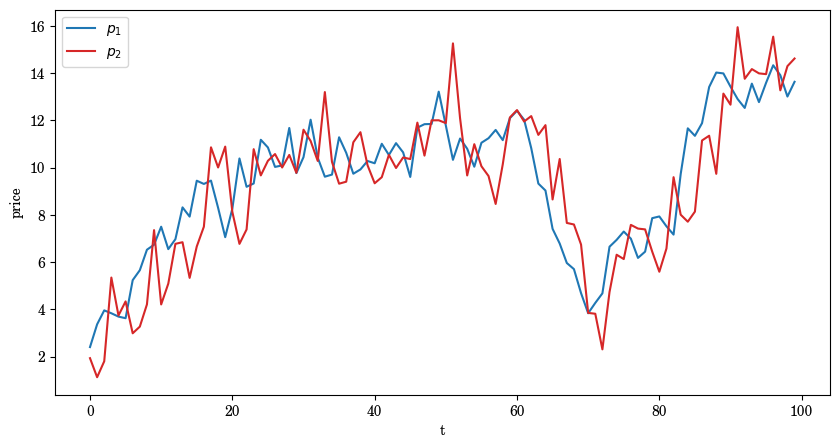
\includegraphics[width=1.0\textwidth]{./images/lagged_walk.png}
    \caption{Lagged random walks. Clearly we see $p_2$ lags behind $p_1$. Note that we only plot $t$ up to 100 for visual clarity.}
\end{figure*}

We derive this result analytically in the following.

Using (\ref{toy1}) and (\ref{toy2}) we get:
\begin{align*}
    \Delta p_{1, t} &= w_{1, t} \\
    \Delta p_{2, t} &= w_{1, t-2} + w_{2, t} - w_{2, t-1}
\end{align*}

Then we can convert to the VMA representation given in (\ref{VMA}):
\[
    \underbrace{
    \begin{bmatrix}
    w_{1,t} \\
    w_{1,t-2} + w_{2,t} - w_{2,t-1}
    \end{bmatrix} 
    }_{= \Delta p}
    =
    \underbrace{
    \begin{bmatrix}
    1 & 0 \\
    L^{2}  & 1 - L
    \end{bmatrix}
    }_{= \Psi(L)}
    \underbrace{
    \begin{bmatrix}
    w_{1,t} \\
    w_{2,t}
    \end{bmatrix}
    }_{=e_t}
.\]

Then recalling that $\Psi(L) = \sum_{k=0}^{\infty} \Psi_k L^k$ 
we have the coefficients:
\begin{align*}
    \Psi(L) =
\underbrace{
\begin{bmatrix}
1 & 0 \\
0 & 1
\end{bmatrix}
}_{:= \Psi_0} L^0
+
\underbrace{
\begin{bmatrix}
0 & 0 \\
0 & -1
\end{bmatrix}
}_{:= \Psi_1} L^1
+
\underbrace{
\begin{bmatrix}
0 & 0  \\
1 & 0
\end{bmatrix}
}_{:= \Psi_2}L^{2}
\end{align*}
Then plugging these into (\ref{Psi1}) we get:
\[
    \Psi(1) = \begin{bmatrix} 1 & 0 \\ 1 & 0 \end{bmatrix} 
.\]
Which has common row vector $\psi := [1 ~ 0]$. Then using (\ref{Hasequation})
and $\Omega = I_2$ we get the Information Share of the first price series to be $1$
and the Information Share of the second series to be $0$, as expected.

% We also examine the case when we have two simple random walks:
%
% \begin{align}
%     p_{1, t} &= p_{1, t-1} + w_{1, t} = \sum_{s=1}^{t} wShare{1, s}\\
%     p_{2, t} &= p_{2, t-1} + w_{2, t} = \sum_{s=1}^{t} w_{2, s}
% \end{align}
%
% \textbf{TODO:} Analytically derive hasbrouck information share for this example.
%
% Where $w_{j, t} \sim N(0, 1)$ i.i.d and $p_0 := 0$.
%
% Clearly this example is co-integrated $I(1)$, since $\mathbb{E}(p_{j,t}) = \sum_{s=1}^{t} \mathbb{E}(w_{j,s}) = 0$ and
% $\text{var}(p_{j, t}) = \sum_{s=1}^{t} \text{var}(w_{j, s}) = t$
% and therefore $\mathbb{E}(\Delta p_t) = \text{var}(\Delta p_t) = 0$.
%
%
% \begin{figure}[htpb]
%     \centering
%     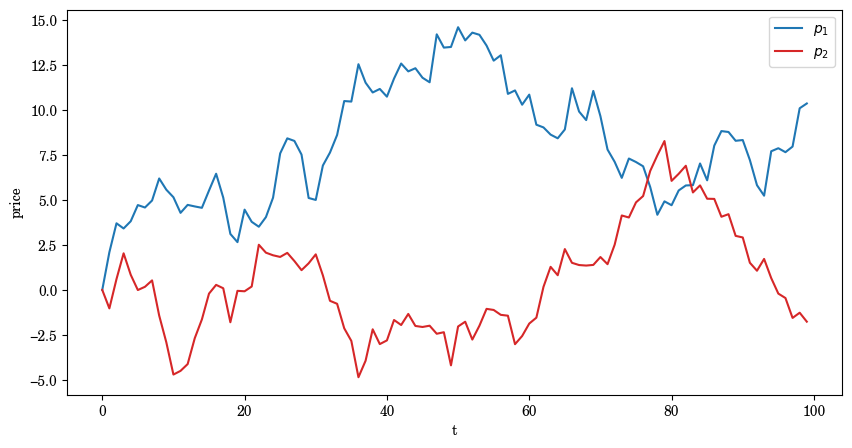
\includegraphics[width=1.0\textwidth]{./images/random_walk.png}
%     \caption{Random walks}
% \end{figure}
%
\section{Orderbook Application}

Following \cite{CAO2009} we resample our data to $1s$ intervals and define the weighted price as:
\begin{equation}
    \text{WP}^{n_{1}, n_{2}} := \frac{\sum_{j=n_{1}}^{n_{2}} q_{j}^B p_{j}^B + q_{j}^A p_{j}^A}{\sum_{j=n_{1}}^{n_{2}} (q^B_{j} + q^A_{j})}
\end{equation}
where $n_{1} \leq n_{2}$. When $n_{1} = n_{2} = 1$ we have the weighted mid-price:
\begin{equation}
    \text{WP}^{1,1} = \frac{q_{1}^B p_{1}^B + q_{1}^A p_{1}^A}{q_{1}^B + q_{1}^A}
\end{equation}

So $\text{WP}^{n_{1},n_{2}}$ is an average price between level $n_{1}$ and $n_{2}$, weighted by volume, encapsulating all the information in the orderbook between levels $n_{1}$ and $n_{2}$ inclusive.

We compare the information content of $\text{WP}^{1,1}$ and $\text{WP}^{2,10}$, i.e how does the information
at the top of the book compare to the other, deeper levels.
So our price series is given by $p_t := (\text{WP}^{1,1}_t, \text{WP}^{2,10}_t)$.
The mid-price and the weighted price have the same common stochastic factor,
are both non-stationary and therefore it is clear that they are $I(1)$ co-integrated.

\begin{figure*}[htpb]
    \centering
    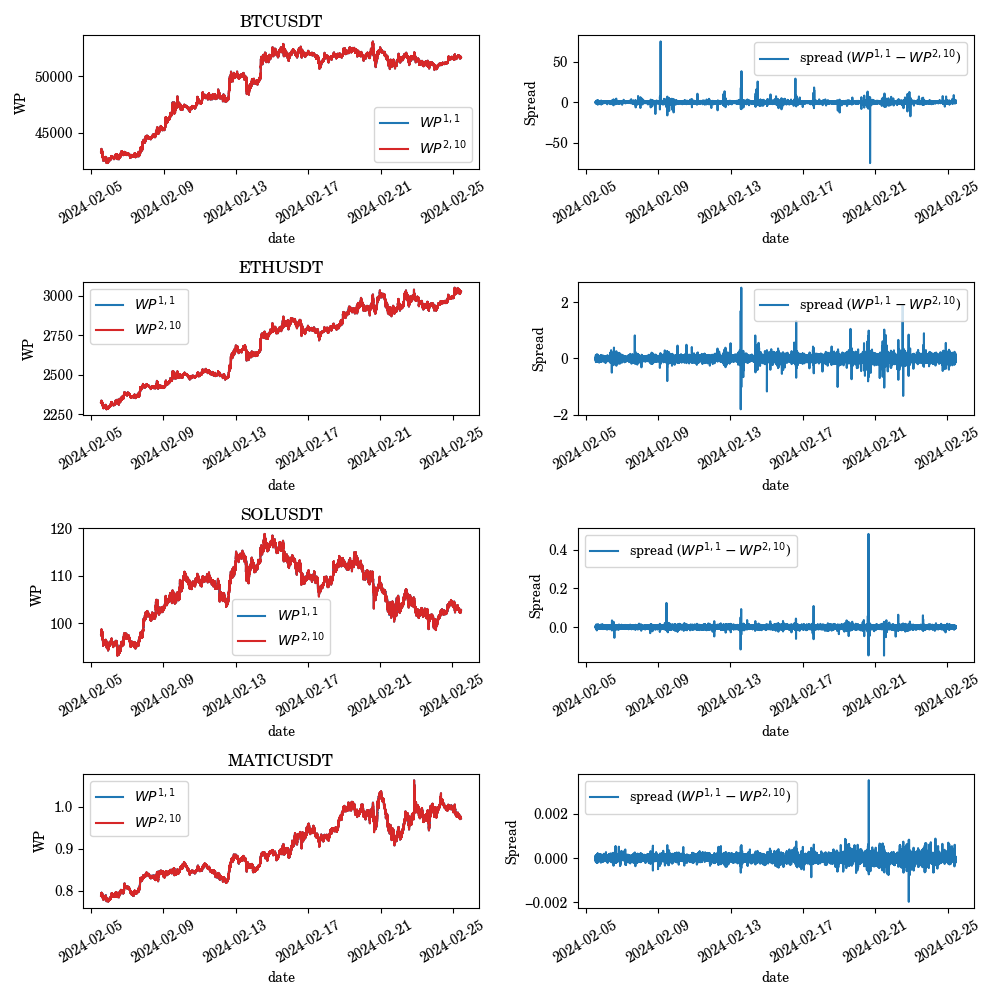
\includegraphics[width=1.0\textwidth]{./images/weighted_prices.png}
    \caption{Weighted prices and their spread for each trading pair.}
    \label{spread}
\end{figure*}

Interestingly we see from Figure \ref{spread} that for our data BTCUSDT
has some very large outlier spreads whereas MATICUSDT seems to be much more stable.
Also we observe that in general across all our trading pairs there is a slight increase
in spread towards the end of the month.


So now we calculate \footnote{Note that when calculating information shares, we have too much data to fit
into memory, so we calculate the information share for windows of size 10,000 and then
we average. Standard deviations are also given in parenthesis.} the Information Share using the estimators we defined above
and report the results in Table \ref{table:1}.

\begin{table}[H]
    \begin{center}
        \begin{tabular}{ccccc}
            \toprule
            trading pair    & $\text{WP}^{1,1}$ Min IS & $\text{WP}^{1,1}$ Max IS & $\text{WP}^{2,10}$ Min IS & $\text{WP}^{2,10}$ Max IS \\
            \midrule
            BTCUSDT   & 0.05 (0.04)  & 0.97 (0.02)   & 0.03 (0.02) & 0.95 (0.04)   \\
            ETHUSDT   & 0.06 (0.05)  & 0.98 (0.03)   & 0.02 (0.03) & 0.94 (0.05)  \\
            SOLUSDT   & 0.08 (0.05)     & 0.98 (0.02)  & 0.02 (0.02) & 0.92 (0.05)   \\
            MATICUSDT &   0.04 (0.06)    & 0.87 (0.12)  & 0.13 (0.12) & 0.96 (0.06)  \\
            \bottomrule
        \end{tabular}
        \caption{IS Results for each trading pair.}
    \label{table:1}
    \end{center}
\end{table}

So we see that for each price series the minimum IS is close to zero and the maximum is close 1.
This is unexpected. For example when \cite{CAO2009} applied the same methodology they
had a much tighter spread between max and min information share for each stock.
This large difference means that for us information share is hard to interpret and 
is perhaps not as useful for this application as one would have hoped.
As \cite{YAN2010} points out, large differences in minimum and maximum Information Share
occur when the residuals, $e_t$ are highly correlated across series.

When we examine our estimated $\Omega$ covariance matrices we find this to be the case.
This implies that the innovations at the top of the orderbook are highly correlated
with the innovations affecting prices further down the orderbook. As \cite{KARABIYIK2022}
points out, these correlations can be partly alleviated by using higher frequency data.
We re-sample our data to 250ms intervals (instead of 1s) and observe a reduction
in covariance. However this reduction is not sufficient and we still observe a large gap in max and min Information Shares.
This is perhaps due to the fact that
for cryptocurrency data the trading is much higher volume and higher frequency
than traditional stocks as studied in \cite{CAO2009}, and so in order for the 
innovations to be uncorrelated, we need much higher frequency sampling.
Since we are limited by our Websocket data to a minimum resolution, we can go no further. 

We conclude that for Binance Websocket data, information shocks
driving price change are highly correlated across orderbook levels.
A consequence of this being that the Hasbrouck Information Share cannot be applied reliably
to measure Information Shares across levels.

